%!TEX TS-program = xelatex
%!TEX encoding = UTF-8 Unicode

\documentclass[a4paper]{article}

\usepackage[bottom]{footmisc}
\usepackage{xltxtra}
\usepackage{amsfonts}
\usepackage{polyglossia}
\usepackage{fancyhdr}
\usepackage{geometry}
\usepackage{dsfont}
\usepackage{amsmath}
\usepackage{amsthm}
\usepackage{amssymb}
\usepackage{physics}
\usepackage{mathtools}
\usepackage{bm}
\usepackage{siunitx}
\usepackage{subcaption}
\usepackage{float}

\usepackage{graphicx}
\graphicspath{ {figures/} }

\usepackage{hyperref}
\hypersetup{
    colorlinks=true,
    linkcolor=blue,
    filecolor=magenta,      
    urlcolor=cyan,
    citecolor=blue,
}
\urlstyle{same}

% Hack to make ieeeconf and natbib get along
% http://newsgroups.derkeiler.com/Archive/Comp/comp.text.tex/2006-02/msg00834.html
\makeatletter
\let\NAT@parse\undefined
\makeatother
\usepackage[numbers]{natbib}
\setcitestyle{aysep={}} % remove comma
\usepackage{usebib}
\bibinput{refs}

\geometry{a4paper,left=15mm,right=15mm,top=20mm,bottom=20mm}
\pagestyle{fancy}
\lhead{Parker C. Lusk}
\chead{Autopilot Estimators}
\rhead{\today}
\cfoot{\thepage}

\setlength{\headheight}{23pt}
% \setlength{\parindent}{0.0in}
\setlength{\parskip}{0.03in}

\newtheorem*{prop}{Proposition}
\newtheorem*{defn}{Definition}
\newtheorem*{thm}{Theorem}
\newtheorem*{cor}{Corollary}
\newtheorem*{lem}{Lemma}
\newtheorem*{rem}{Remark}

\DeclarePairedDelimiterX{\inn}[2]{\langle}{\rangle}{#1, #2}

\begin{document}
\section*{Overview}
High-level autonomy requires confidence in low-level control and estimation.
Autopilot firmware can use an inertial measurement unit (IMU) with three orthogonal rate gyroscopes and three orthogonal accelerometers to perform estimation.
If sensors were perfect, the estimator would simply integrate the gyro measurements to obtain an estimate of the attitude.
However, gyros tend to drift over time due to bias.
The accelerometer can be used to correct the drift in the roll and pitch axes, however yaw bias is unobservable with an IMU alone.
This document explores various schemes and implementations of attitude estimation using an IMU, with occasional external attitude updates from vision, motion capture, or some other source.
Another good reference is~\cite{Kok2017}.

\section*{IMU Model}
With the advent of micro electro-mechanical systems (MEMS), the scale of IMUs has decreased significantly over the years.
In particular, the spread of small MEMS IMUs is in part due to the proliferation of smart phones and wearable electronics.

To understand the IMU model, consider a rigid body $\{B\}$ with a position $\bm{r}$ expressed in an inertial frame $\{A\}$.
An IMU is `strapped down' to the origin of the rigid body and is axis aligned with it.
In other words, the IMU sensor frame $\{S\}$ is identified with the body frame $\{B\}$.
Unless otherwise stated, we will make use of the East-North-Up (ENU) inertial frame with its corresponding Front-Left-Up (FLU) body frame.
The rotation matrix $R^A_B$ is the local-to-global rotation of $\{B\}$ w.r.t $\{A\}$ and it takes data from $\{B\}$ into $\{A\}$.
The bases (axes) of $\{A\}$ are written $\{\bm{e}_i\}$.

With this problem geometry, we write the measurements received by the IMU below.

\subsection*{Accelerometer}
Accelerometers do not measure gravity.
Instead, an accelerometer measures the \textit{specific force} (i.e., $\bm{F}/m$) that prevents free fall.
Thus, an accelerometer free falling in a vacuum would measure $0$, while an accelerometer sitting on a table would measure the normal force that is preventing free fall.
The measurement equation is
\begin{equation}
  \bm{a} = \left(R^A_B\right)^\top (\ddot{\bm r} + g\bm{e}_3) + \bm{\nu} + \bm{b}_a,
\end{equation}
where $g\approx\SI{9.81}{\meter\per\second^2}$, $\bm{\nu}$ is zero-mean Gaussian noise with variance $\Sigma^2_a$ and $\bm{b}_a$ is a bias term.
Note that it may seem contrary to have \textit{plus} $g\bm{e}_3$, but this is correct since we are working in an ENU/FLU frame, where gravity is actually $-g\bm{e}_3$; therefore, we are actually \textit{subtracting} the gravity acceleration vector.

MEMS accelerometers often have a sample rate of 100 Hz to 1 kHz.

\subsection*{Rate Gyro}
The measured angular rate $\bm{\omega} = \begin{bmatrix}p&q&r\end{bmatrix}^\top$ is the body rate of the vehicle with respect to the inertial frame, expressed in the body frame and is written as
\begin{equation}
  \bm{\omega} = \bm{\omega}_\text{true} + \bm{\eta} + \bm{b},
\end{equation}
where $\bm{\eta}$ is zero-mean Gaussian noise with variance $\Sigma^2_\omega$ and $\bm{b}$ is constant or slowly time-varying bias (i.e., $\dot{\bm b}\approx 0)$.

Gyros typically have a sample rate of 500 Hz, 1 kHz, or 8 kHz.
They are great at capturing high-frequency dynamics and are incredibly useful, especially over short time windows.
However, due to the low-frequency bias $\bm{b}$, simply integrating gyros over long timescales is unwise (e.g., more than tens of seconds).

\subsubsection*{Allan Variance}
\subsubsection*{AR(n) Model}

\section*{Linear Complementary Filter}
One of the most basic estimators is the \textit{complementary filter}, also known as the \textit{balance filter} (Shane Colton, 2007).
The motivating principle is that gyros are good at capturing high-frequency dynamics, but have a low-frequency drift.
On the otherhand, accelerometers tend to have high-frequency noise (e.g., from non-smooth movement).
Further, when the system that the IMU is attached to has actuators (like a multirotor), 

As indicated above, complementary filters are useful for fusing independent noisy measurements of the same signal with complementary spectral characteristics.
Here, we give an overview of the theory of complementary filters and derive a linear estimator for a kinematic dynamic process with constant bias.
This theoretical overview follows the discussion in Appendix A of~\citet{Mahony2008}.

\subsection*{Estimation for Static System}
Consider a time-varying signal $x(t)$ we wish to observe.
We have two sensors $y_1$ and $y_2$ that measure the signal with additive noise
\begin{equation}
\begin{split}
y_1(t) &= x(t) + \mu_1(t) \\
y_2(t) &= x(t) + \mu_2(t)
\end{split}
\qquad\qquad\qquad
\begin{split}
\mu_1 &\rightarrow \text{high-frequency noise/disturbance} \\
\mu_2 &\rightarrow \text{low-frequency noise/disturbance}
\end{split}
\end{equation}
Given that we know the noises are complementary in a spectral sense, we can design a pair of complementary transfer functions, $F_1(s) + F_2(s) = 1$, to filter out the noise while allowing the signal to pass.
Filtering each measurement through its corresponding transfer function results in the estimate
\begin{align}
\hat{x}(s) &= F_1(s)y_1(s) + F_2(s)y_2(s) \nonumber \\
           &= F_1(s)\left[x(s) + \mu_1(s)\right] + F_2(s)\left[x(s) + \mu_2(s)\right] \label{eq:scf_estimator} \\
           &= (F_1(s)+F_2(s))x(s) + F_1(s)\mu_1(s) + F_2(s)\mu_2(s) \nonumber \\
           &= x(s) + F_1(s)\mu_1(s) + F_2(s)\mu_2(s), \label{eq:scf_estimate}
\end{align}
where we construct $F_1(s)$ to be low-pass and $F_2(s)$ to be high-pass to appropriately filter out the known spectral content of the disturbances.
Notice that $x(s)$ is all-pass as desired.
Recall that a first-order low-pass filter has the frequency response
\begin{equation}
H_\text{LPF}(s) = \frac{\omega_c}{s+\omega_c} = \frac{1}{\tau s+1};\qquad\tau=\frac{1}{\omega_c}.
\end{equation}
The complement of a LPF is a high-pass filter
\begin{equation}
H_\text{HPF}(s) = 1 - H_\text{LPF}(s) = \frac{s}{s+\omega_c} = \frac{\tau s}{\tau s+1}.
\end{equation}
Thus, by letting $F_1(s)=H_\text{LPF}(s)$ and $F_2(s)=H_\text{HPF}(s)$, we obtain the desired frequency characteristics.

\subsubsection*{Sampled-Data Implementation}
While equation~\eqref{eq:scf_estimate} is useful for analysis, we would like to be able to implement this filter as an algorithm in a digital computer.
This requires implementing equation~\eqref{eq:scf_estimator}, which uses the measurements $y_1$ and $y_2$.
Here, we will discuss two\footnote{A third way uses the bilinear transform to move from the Laplace domain to the Z-domain, followed by the inverse Z transform.} sampled-data implementations of the vanilla linear complementary filter.
Both versions start with using the inverse Laplace transform to rewrite equation~\eqref{eq:scf_estimator} as differential equations.
Once in the time domain, we can perform a zero-order hold on the solution to the differential equation.
Alternatively, an approximation method can be used such as Euler's method, avoiding the necessity of solving the differential equation.

First, we start with the inverse Laplace transform, starting from equation~\eqref{eq:scf_estimator}
\begin{align*}
            \hat{x}(s) &= \frac{\omega_c}{s+\omega_c}y_1(s) + \frac{s}{s+\omega_c}y_2(s) \\
(s+\omega_c)\hat{x}(s) &= \omega_c y_1(s) + s y_2(s) \\
           s\hat{x}(s) &= s y_2(s) + \omega_c \left(y_1(s) - \hat{x}(s)\right),
\end{align*}
which becomes
\begin{equation}\label{eq:scf_with_dot}
\dot{\hat x}(t) = \dot{y}_2(t) + \omega_c\left(y_1(t) - \hat{x}(t)\right).
\end{equation}
Note that how this is written, it appears to be a pair of coupled first-order differential equations.
However, we do not actually know how $y_2(t)$ evolves, and we are interested in the value of the derivative at time $t$, which we can obtain via numerical differentiation.
For clarity, we will define $y_2^\Delta(t):=\dot{y}_2(t)$, leaving us with
\begin{equation}
\dot{\hat x}(t) = -\omega_c\hat{x}(t) + \omega_cy_1(t) + y_2^\Delta(t).
\end{equation}

\textbf{1) ZOH.} The zero-order hold method involves solving the differential equation.
This is not difficult and is left as an exercise to the reader (see Chapter 4.1 of \citet{Beard2017}).

\textbf{2) Approximation via Euler's Method.} In this case, we approximate the time derivative using the limit definition, giving us
\begin{align*}
\frac{\hat{x}_i - \hat{x}_{i-1}}{\Delta t} &= -\omega_c\hat{x}_{i} + \omega_cy_{1,i} + \frac{y_{2,i} - y_{2,i-1}}{\Delta t} \\
\hat{x}_i &=  -\Delta t\omega_c\hat{x}_{i} + \Delta t \omega_c y_{1,i} + y_{2,i} - y_{2,i-1} + \hat{x}_{i-1} \\
(1+\Delta t\omega_c)\hat{x}_i &=  \Delta t \omega_c y_{1,i} + y_{2,i} - y_{2,i-1} + \hat{x}_{i-1} \\
\hat{x}_i &=  \frac{1}{1+\Delta t\omega_c} \left(\Delta t \omega_c y_{1,i} + y_{2,i} - y_{2,i-1} + \hat{x}_{i-1}\right) \\
          &=  \frac{\Delta t \omega_c}{1+\Delta t\omega_c} y_{1,i} + \frac{1}{1+\Delta t\omega_c}\left(y_{2,i} - y_{2,i-1}\right) + \frac{1}{1+\Delta t\omega_c} \hat{x}_{i-1}.
\end{align*}
We can write this compactly as
\begin{equation}
\hat{x}_i = \alpha\hat{x}_{i-1} + \alpha\left(y_{2,i} - y_{2,i-1}\right) + (1-\alpha)y_{1,i},
\end{equation}
where
\begin{equation*}
\begin{split}
\alpha := \frac{1}{1+\Delta t\omega_c} = \frac{\tau}{\tau+\Delta t}
\end{split};
\qquad\qquad
\begin{split}
1-\alpha := \frac{\Delta t\omega_c}{1+\Delta t\omega_c} = \frac{\Delta t}{\tau+\Delta t}
\end{split};
\qquad\qquad
\begin{split}
0\le\alpha\le1
\end{split}.
\end{equation*}
Note that we could have gotten to the same equation by deriving the $\alpha$-LPF and $\alpha$-HPF variants and summing them.

\subsubsection*{Example}
In this example, we use a sample period of $T_s=\SI{0.001}{\second}$ and take $x(t)=\cos(2\pi f_x t)$, where $f_x=\SI{5}{\Hz}$.
The disturbances $\mu_1$ and $\mu_2$ are specified as sinusoids with frequencies $20$ times higher and lower, respectively.
The results are shown in Fig.~\ref{fig:scf_est} for filters designed with a cut-off frequency of $f_c=\SI{1}{\Hz}$ (top) and $f_c=\SI{10}{\Hz}$ (bottom).
The frequency responses of the two filter designs are shown in Fig.~\ref{fig:scf_bode}, in terms of the complementary filters $F_1(s)$ and $F_2(s)$.

Note how varying the cut-off frequency $f_c$ changes the response of the filter, choosing between rejecting more low-frequency or high-frequency noise.
Because of the characteristics of the first-order filters used, the transition band is quite wide.
This results in noise leakage into the estimate when the frequency of the true signal is close to the frequencies of the noise.
By increasing the ratio of the frequencies, we are able to reconstruct $x(t)$ perfectly.

Specifically, when the cut-off frequency is close to the low-frequency disturbance ($\mu_2$), high-frequency noise is heavily attenuated, but low-frequency noise is not as much.
The opposite holds true when the cut-off frequency is close to the high-frequency disturbance ($\mu_1$).
This translates to a choice of $\alpha$ small ($f_c$ large) allowing more high-frequency noise, while $\alpha$ large ($f_c$ small) allows more low-frequency noise.

\begin{figure}[h]
  \centering
  \begin{subfigure}[t]{0.32\textwidth}
    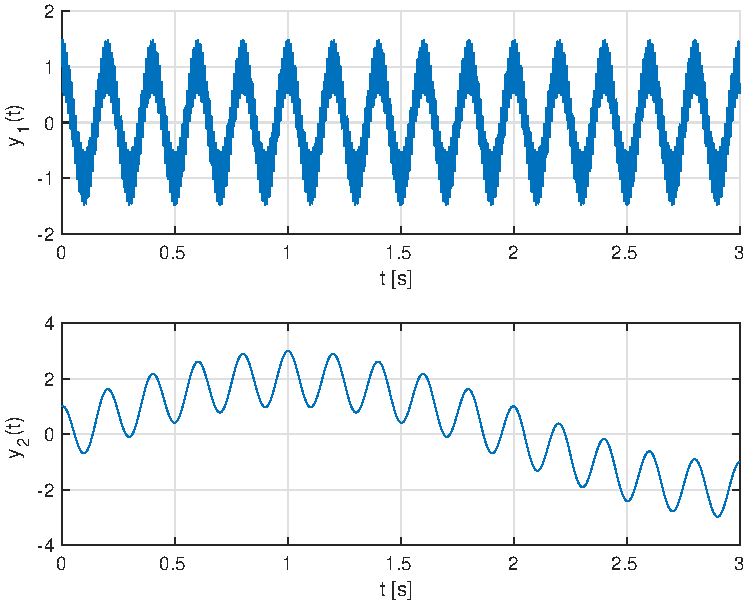
\includegraphics[width=\textwidth]{scf_meas.pdf}
    \caption{Measurements of $x(t)$.}
    \label{fig:scf_meas}
  \end{subfigure}\hfill
  \begin{subfigure}[t]{0.32\textwidth}
    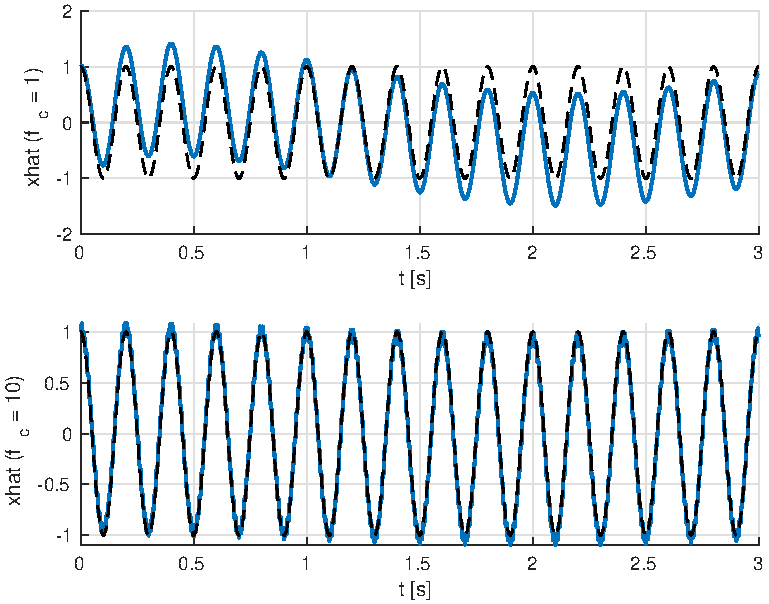
\includegraphics[width=\textwidth]{scf_est.pdf}
    \caption{Estimates using different $\omega_c=2\pi f_c$. The true signal $x(t)$ is shown as the dashed black line.}
    \label{fig:scf_est}
  \end{subfigure}\hfill
  \begin{subfigure}[t]{0.32\textwidth}
    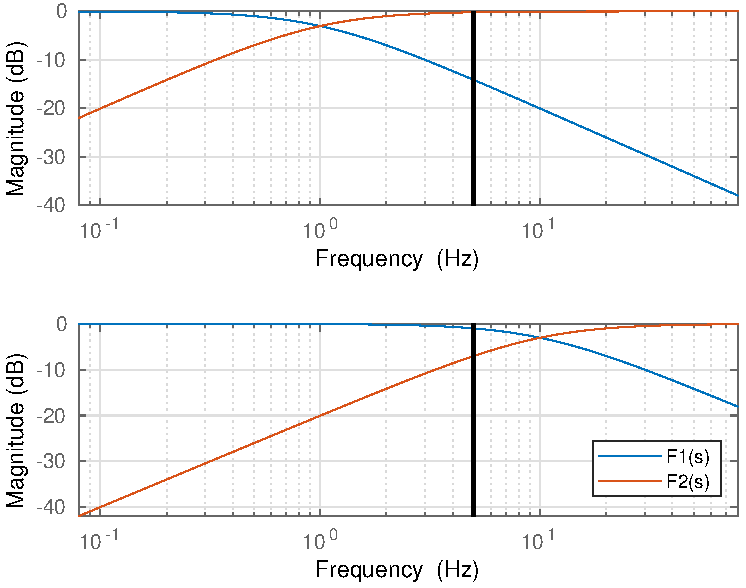
\includegraphics[width=\textwidth]{scf_bode.pdf}
    \caption{Bode magnitude plots of $F_1, F_2$ for different $\omega_c$. The true signal frequency is shown as the thick black vertical line.}
    \label{fig:scf_bode}
  \end{subfigure}
  \caption{Results from an example complementary filter applied to simulated data.}
  \label{fig:scf}
\end{figure}

\subsection*{Estimation for Kinematic System with Bias}
From equation~\eqref{eq:scf_with_dot}, it is clear to see how amenable the complementary filter is to position estimation of a kinematic system.
In particular, notice that the filter uses direct measurements and rate measurements of the unknown signal.
Consider the kinematic model
\begin{equation}\label{eq:kinematic_model}
\dot{x} = u,
\end{equation}
with two sensors that measure
\begin{equation}
\begin{split}
y_x(t) = L(t)*x(t) + \mu_x(t)
\end{split},
\quad
\begin{split}
y_u(t) = u(t) + \mu_u(t) + b(t)
\end{split},
\end{equation}
where $L(t)$ is the impulse response of a low-pass filter associated with sensor characteristics, $L*x$ denotes convolution, $\mu$ represents noise in both measurements, and $b(t)$ is a deterministic perturbation that is dominated by low-frequency content.
Normally $L(s)\approx1$ over the frequency range on which the measurement $y_x$ is of interest~\cite{Mahony2008}.
The rate measurement $y_u(t)$ is integrated as $y_u(s)/s$ to obtain an estimate of the state and the noise and bias characteristics of the integrated signal are dominated by low-frequency content.

To add flexibility to our design, we choose
\begin{equation}
\begin{split}
F_1(s) := \frac{C(s)}{s + C(s)}
\end{split},
\qquad
\begin{split}
F_2(s) := 1 - F_1(s) = \frac{s}{s + C(s)}
\end{split},
\end{equation}
with $C(s)$ all-pass so that $L(s)F_1(s)\approx1$ over the bandwidth of $L(s)$ (while $F_2(s)\ll1$).
Thus,
\begin{align}
\hat{x}(s) &= F_1(s)y_x(s) + F_2(s)\frac{y_u(s)}{s} \nonumber \\
           &= F_1(s)\left[L(s)x(s) + \mu_x(s)\right] + F_2(s)\frac{1}{s}\left[u(s) + \mu_u(s) + b(s)\right] \nonumber \\
           &= (F_1(s)L(s)+F_2(s))x(s) + F_1(s)\mu_x(s) + F_2(s)\frac{1}{s}\left[\mu_u(s) + b(s)\right] \nonumber \\
           &\approx x(s) + F_1(s)\mu_x(s) + F_2(s)\frac{1}{s}\left[\mu_u(s) + b(s)\right].
\end{align}

\section*{Mahony's Nonlinear Complementary Filter}
One of the more popular estimators is Mahony's nonlinear complementary filter on $\mathrm{SO}(3)$~\cite{Mahony2008}.

\begin{align}
  \dot{\bm{\hat{q}}} &= \frac{1}{2} \hat{\bm q} \otimes \bm{\bar \omega} \\
  \dot{\bm{\bar \omega}} &= (\bm{\omega} - \bm{b}) + k_P\bm{\omega}_\text{err} \\
  \dot{\bm{b}} &= -k_I\bm{\omega}_\text{err}
\end{align}

\begin{align}
  \bm{\omega}_\text{err} = \sum v_i \times \hat{v}_i
\end{align}

\begin{align}
  \tilde{\bm{q}} &= \hat{\bm q}^{-1} \otimes \bm{q}(\bm{a}) \\
  \bm{\omega}_\text{err} &= 2 q_w \bm{q}_\text{vec}
\end{align}

\section*{Autopilot Implementation}
The Mahony filter is implemented for experimental validation on IMU data.
We also incorporate a strategy for implementing external attitude corrections (e.g., from VICON or VIO).



\subsection*{Experimental Results}

\begin{figure}[H]
  \centering
  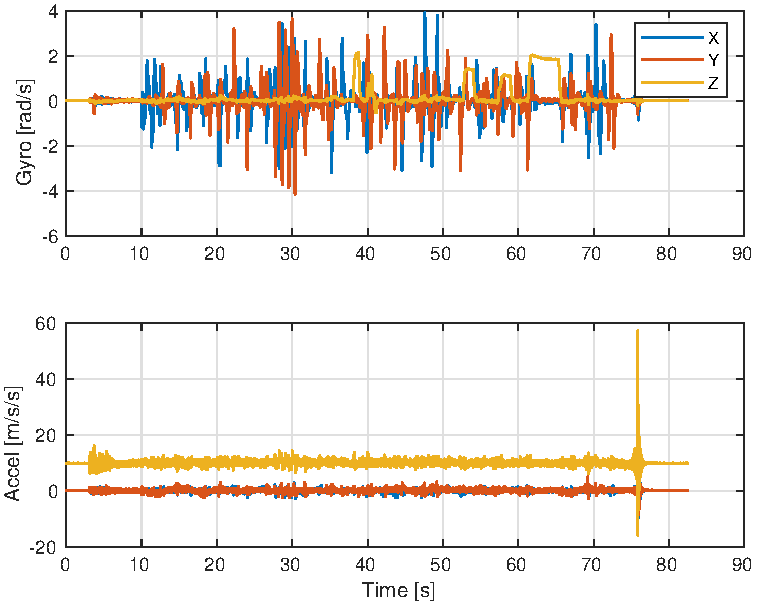
\includegraphics[width=0.5\textwidth]{rawimu.pdf}
  \caption{Raw IMU data from non-aggressive HX02 flight.}
  \label{fig:rawimu}
\end{figure}

\subsubsection*{Test 1 - Gyro Only}

\begin{figure}[H]
  \centering
  \begin{subfigure}[t]{0.31\textwidth}
    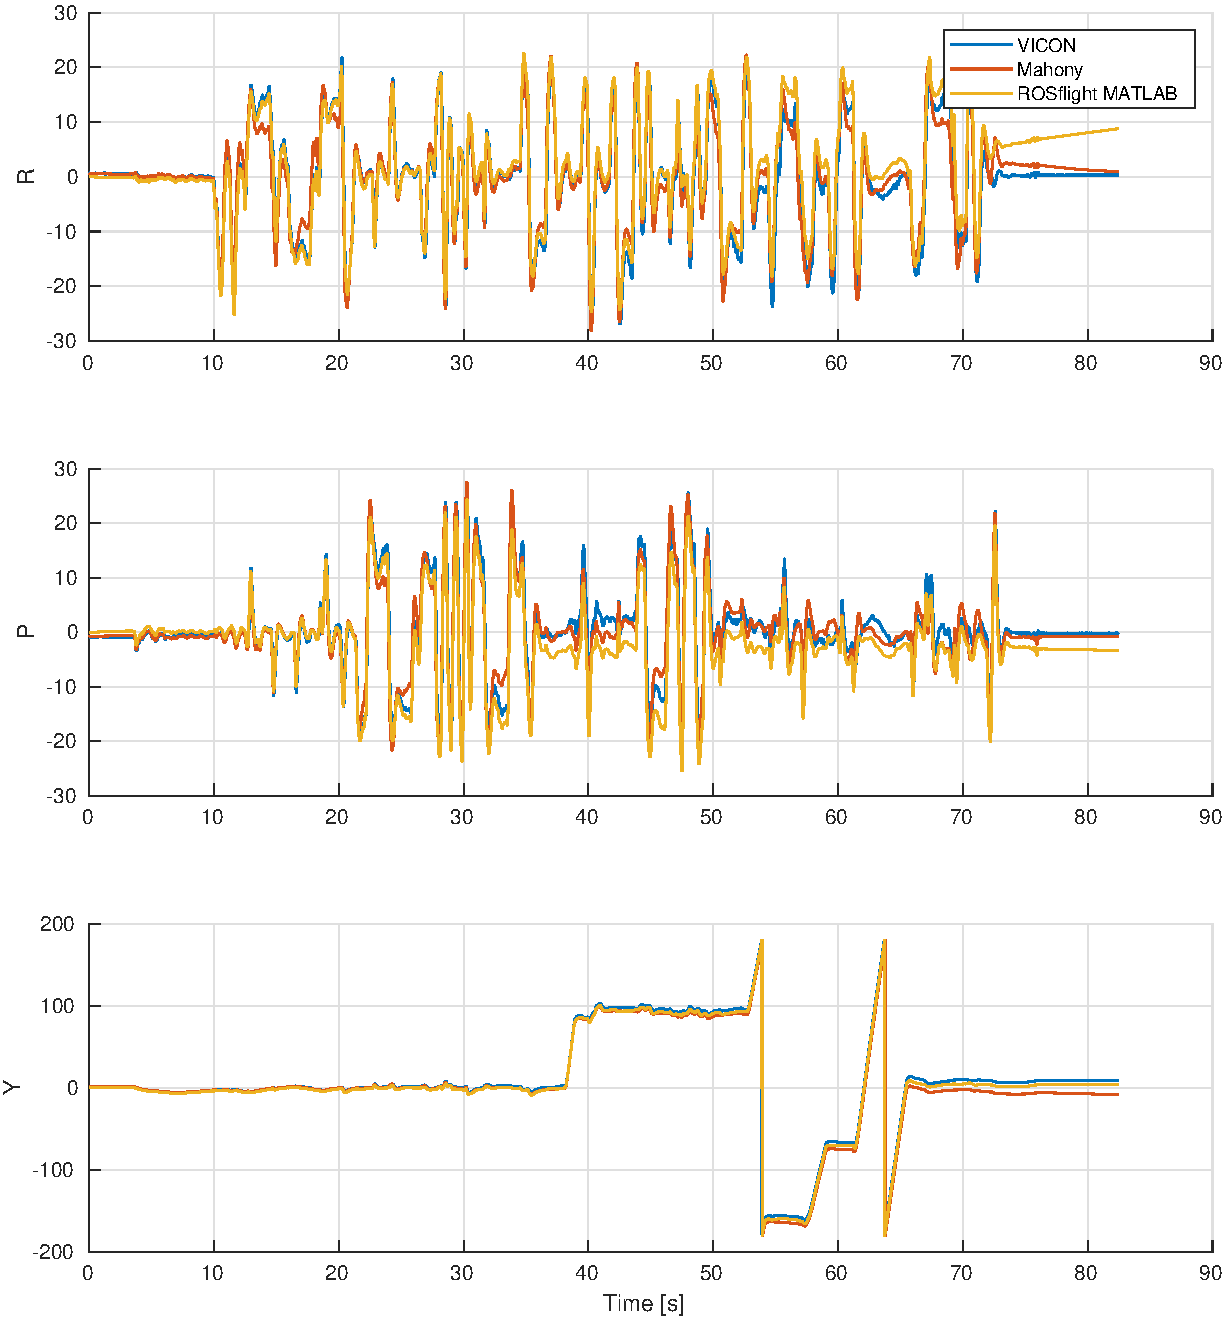
\includegraphics[width=\textwidth]{estrpy_gyroonly.pdf}
    \caption{RPY estimates}
    \label{fig:scf_meas}
  \end{subfigure}\hfill
  \begin{subfigure}[t]{0.31\textwidth}
    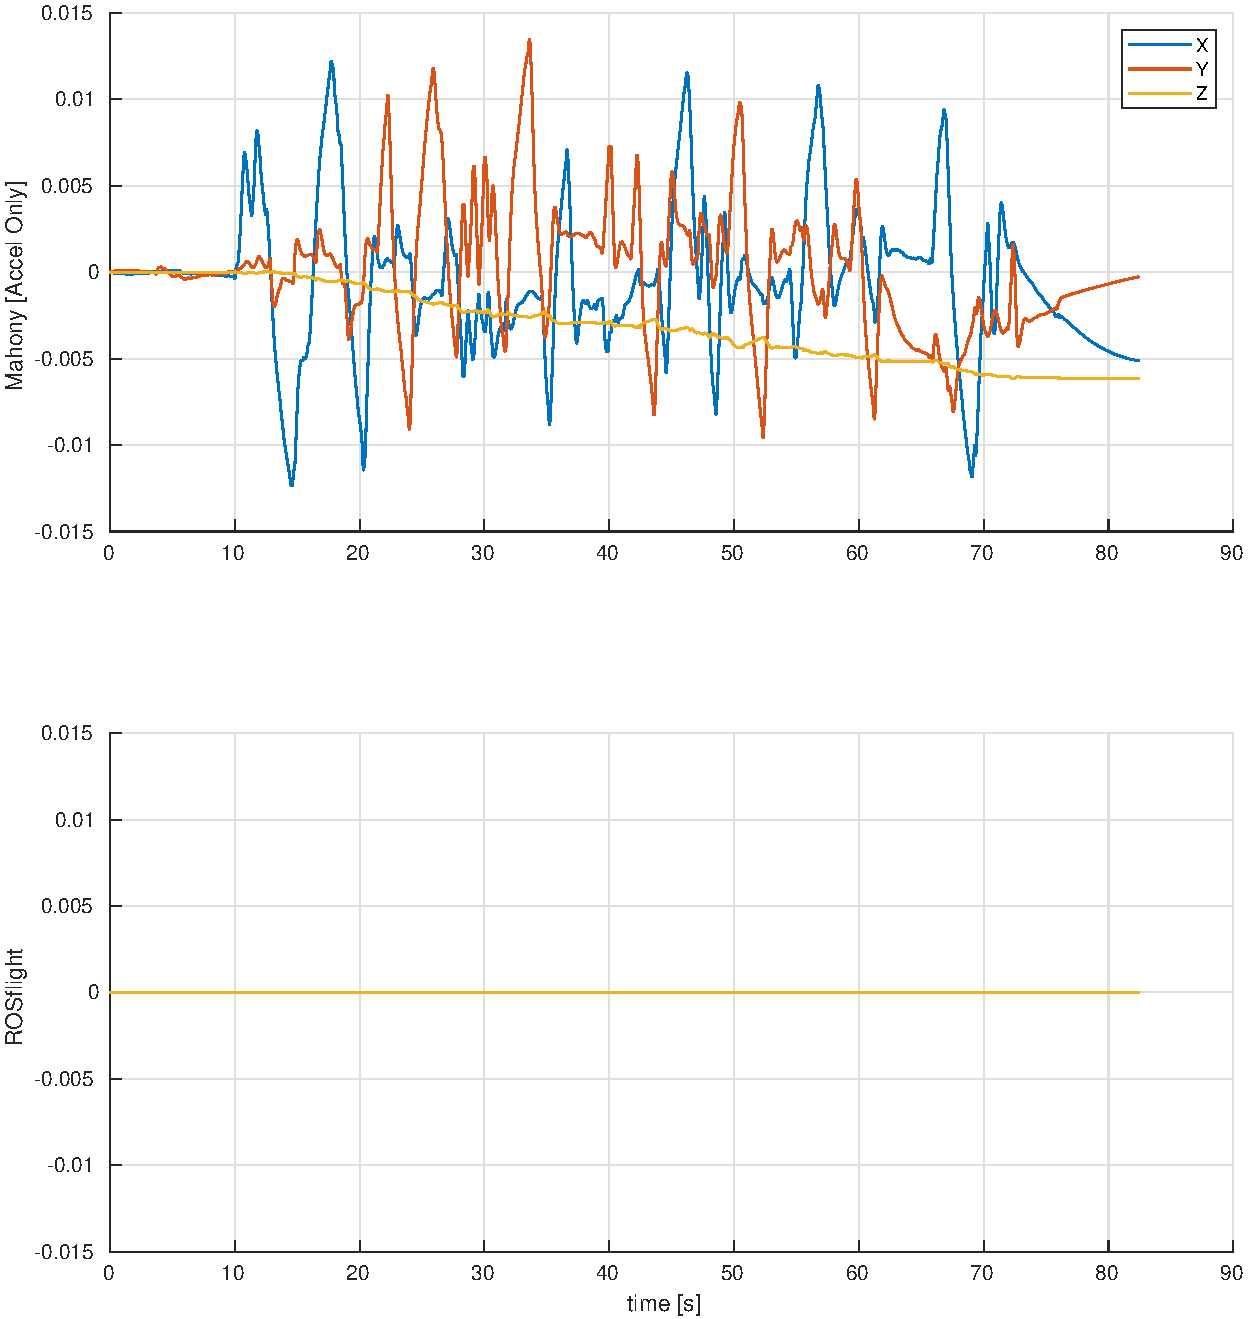
\includegraphics[width=\textwidth]{estbias_gyroonly.pdf}
    \caption{Bias estimates}
    \label{fig:scf_est}
  \end{subfigure}\hfill
  \begin{subfigure}[t]{0.31\textwidth}
    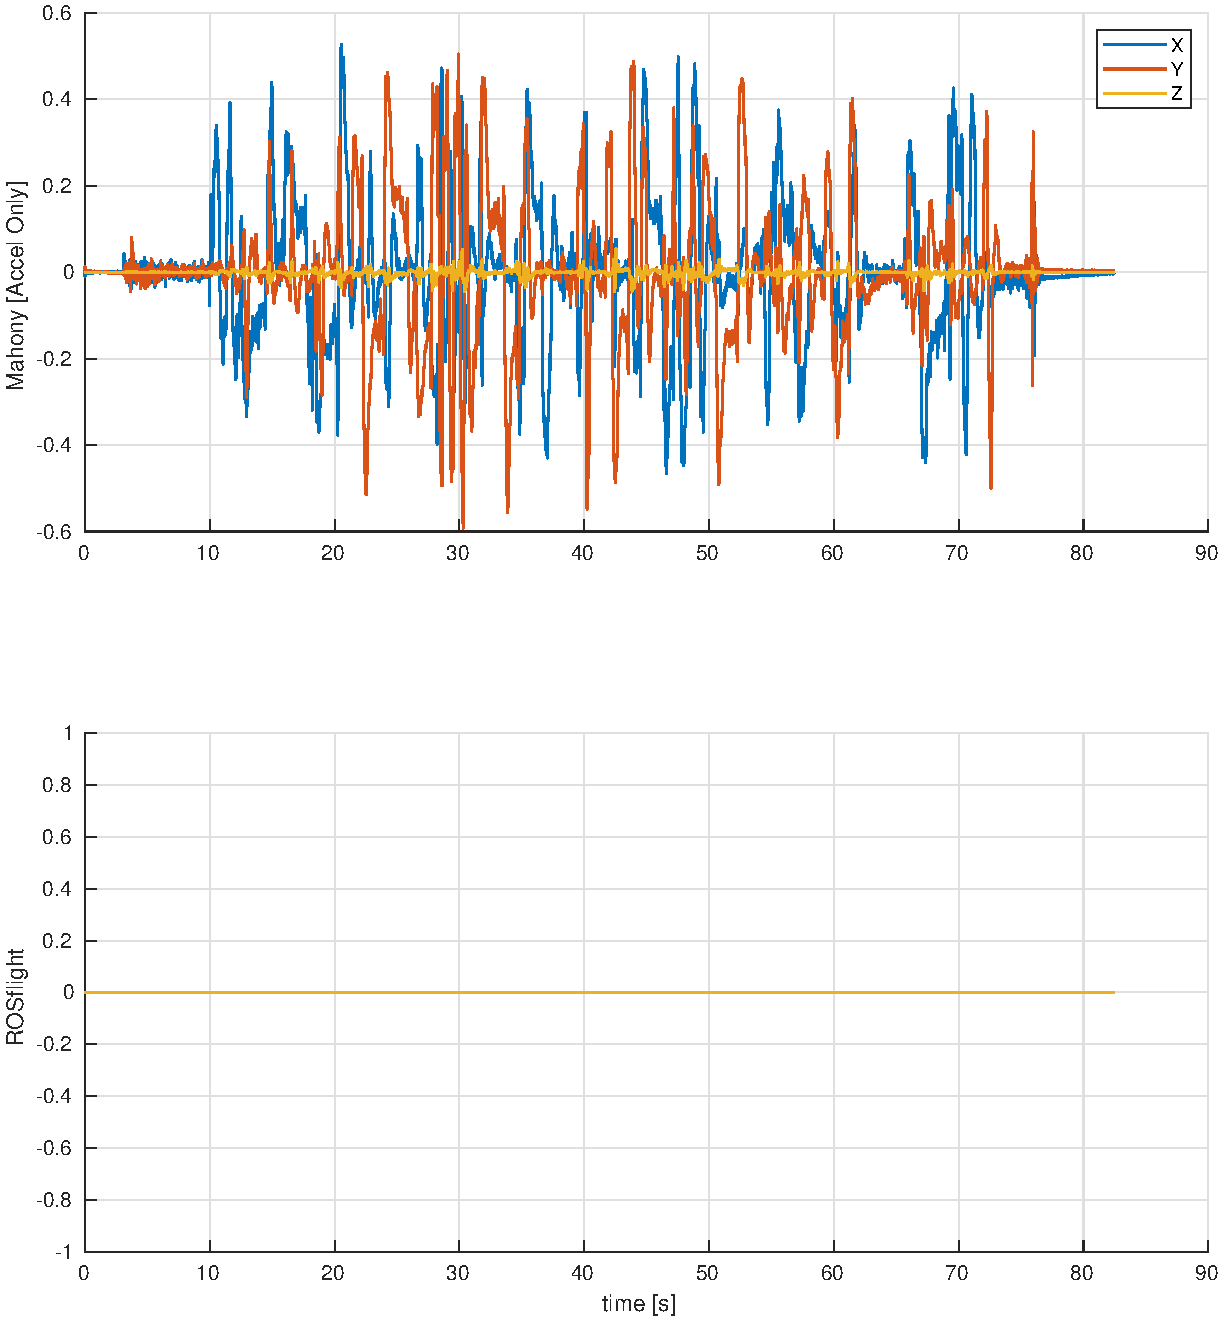
\includegraphics[width=\textwidth]{werr_gyroonly.pdf}
    \caption{$\omega_\text{err}$}
    \label{fig:scf_bode}
  \end{subfigure}
  \caption{Results from Test 1.}
  \label{fig:scf}
\end{figure}

\subsubsection*{Test 2 - Gyro + External Attitude at 100 Hz}

\begin{figure}[H]
  \centering
  \begin{subfigure}[t]{0.31\textwidth}
    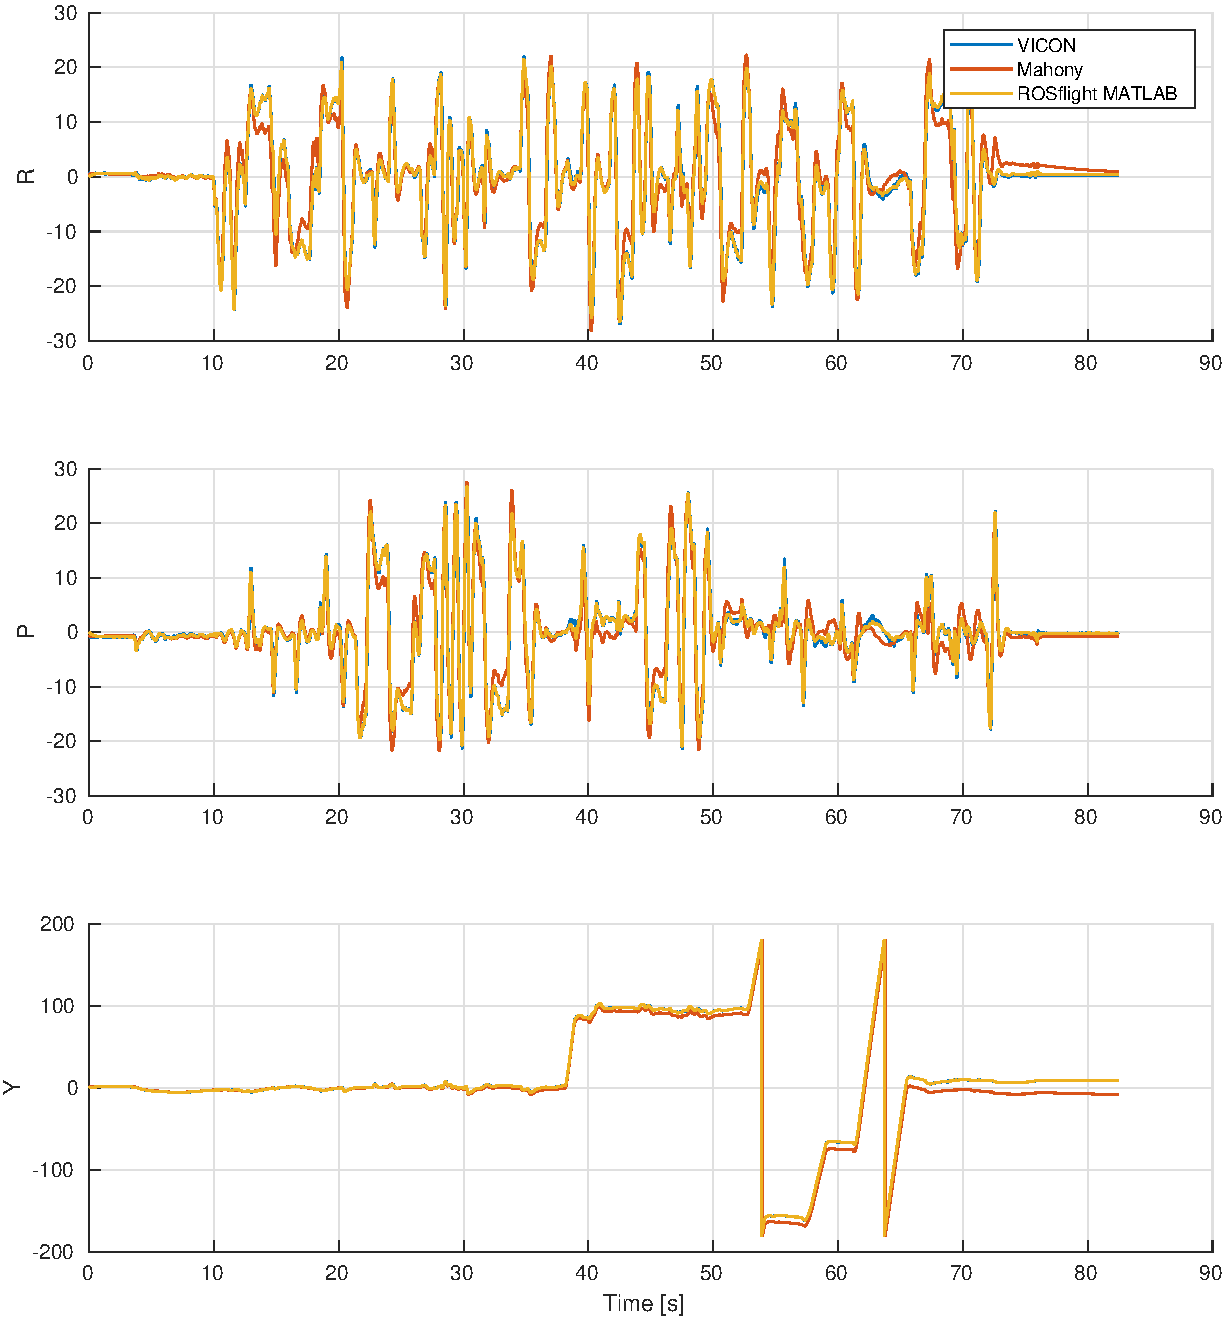
\includegraphics[width=\textwidth]{estrpy_ext100.pdf}
    \caption{RPY estimates}
    \label{fig:scf_meas}
  \end{subfigure}\hfill
  \begin{subfigure}[t]{0.31\textwidth}
    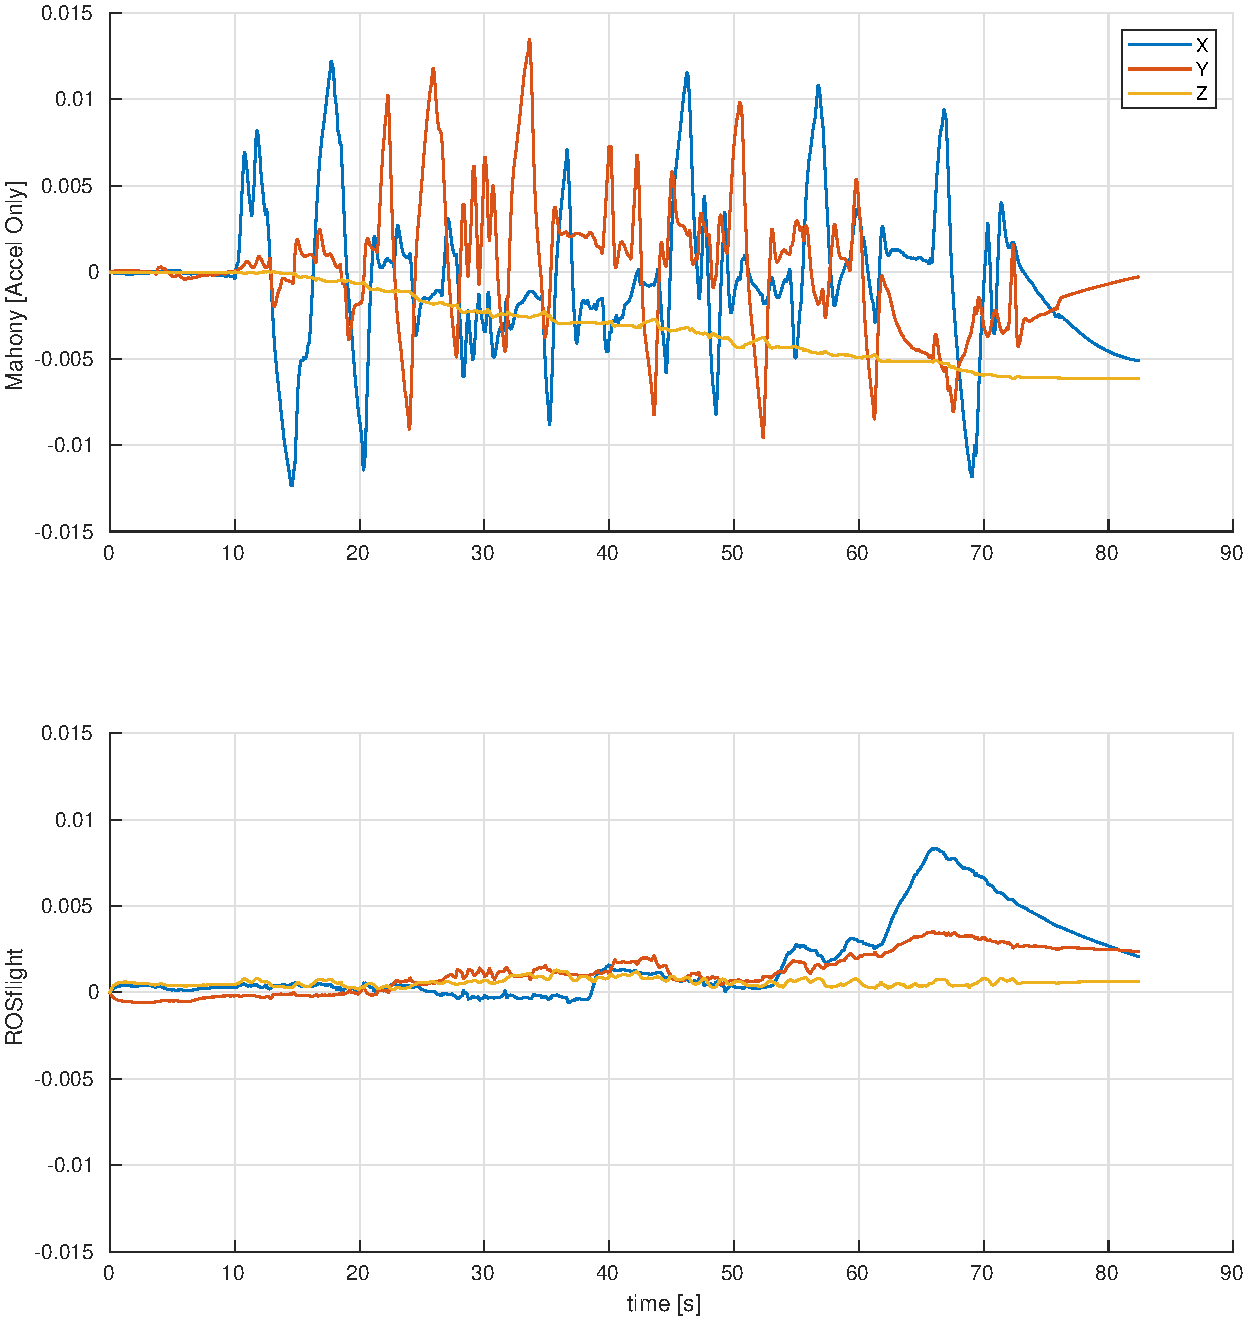
\includegraphics[width=\textwidth]{estbias_ext100.pdf}
    \caption{Bias estimates}
    \label{fig:scf_est}
  \end{subfigure}\hfill
  \begin{subfigure}[t]{0.31\textwidth}
    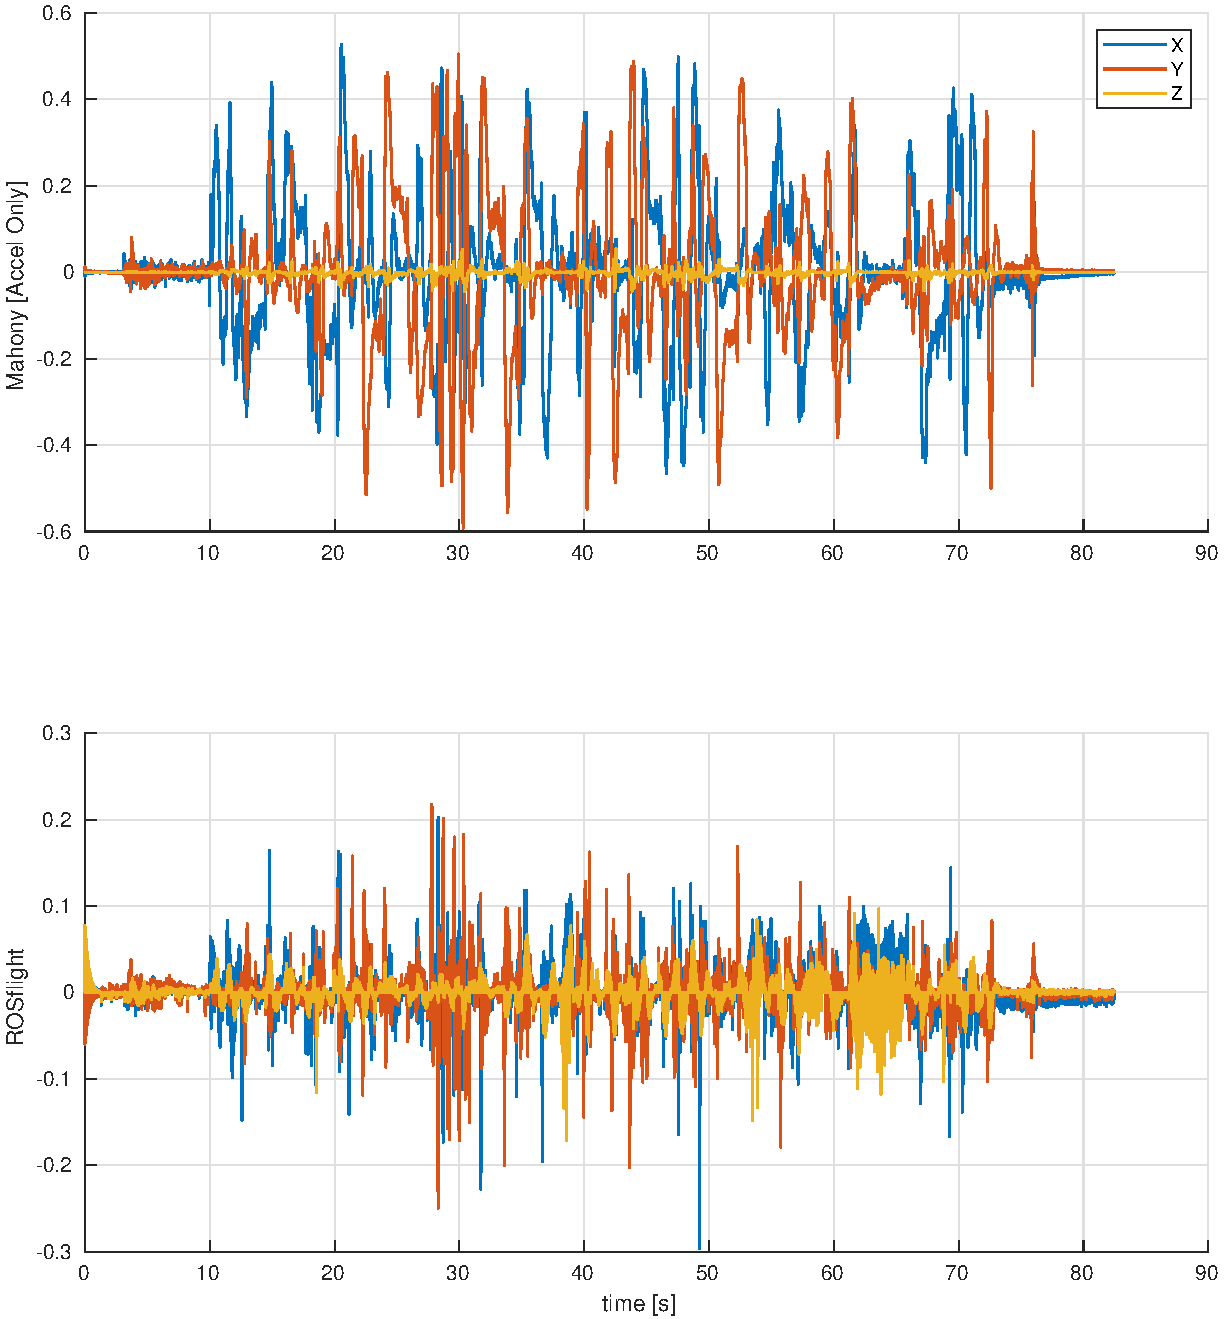
\includegraphics[width=\textwidth]{werr_ext100.pdf}
    \caption{$\omega_\text{err}$}
    \label{fig:scf_bode}
  \end{subfigure}
  \caption{Results from Test 2.}
  \label{fig:scf}
\end{figure}

\subsubsection*{Test 3 - Gyro + Accel + External Attitude at 100 Hz}

\begin{figure}[H]
  \centering
  \begin{subfigure}[t]{0.31\textwidth}
    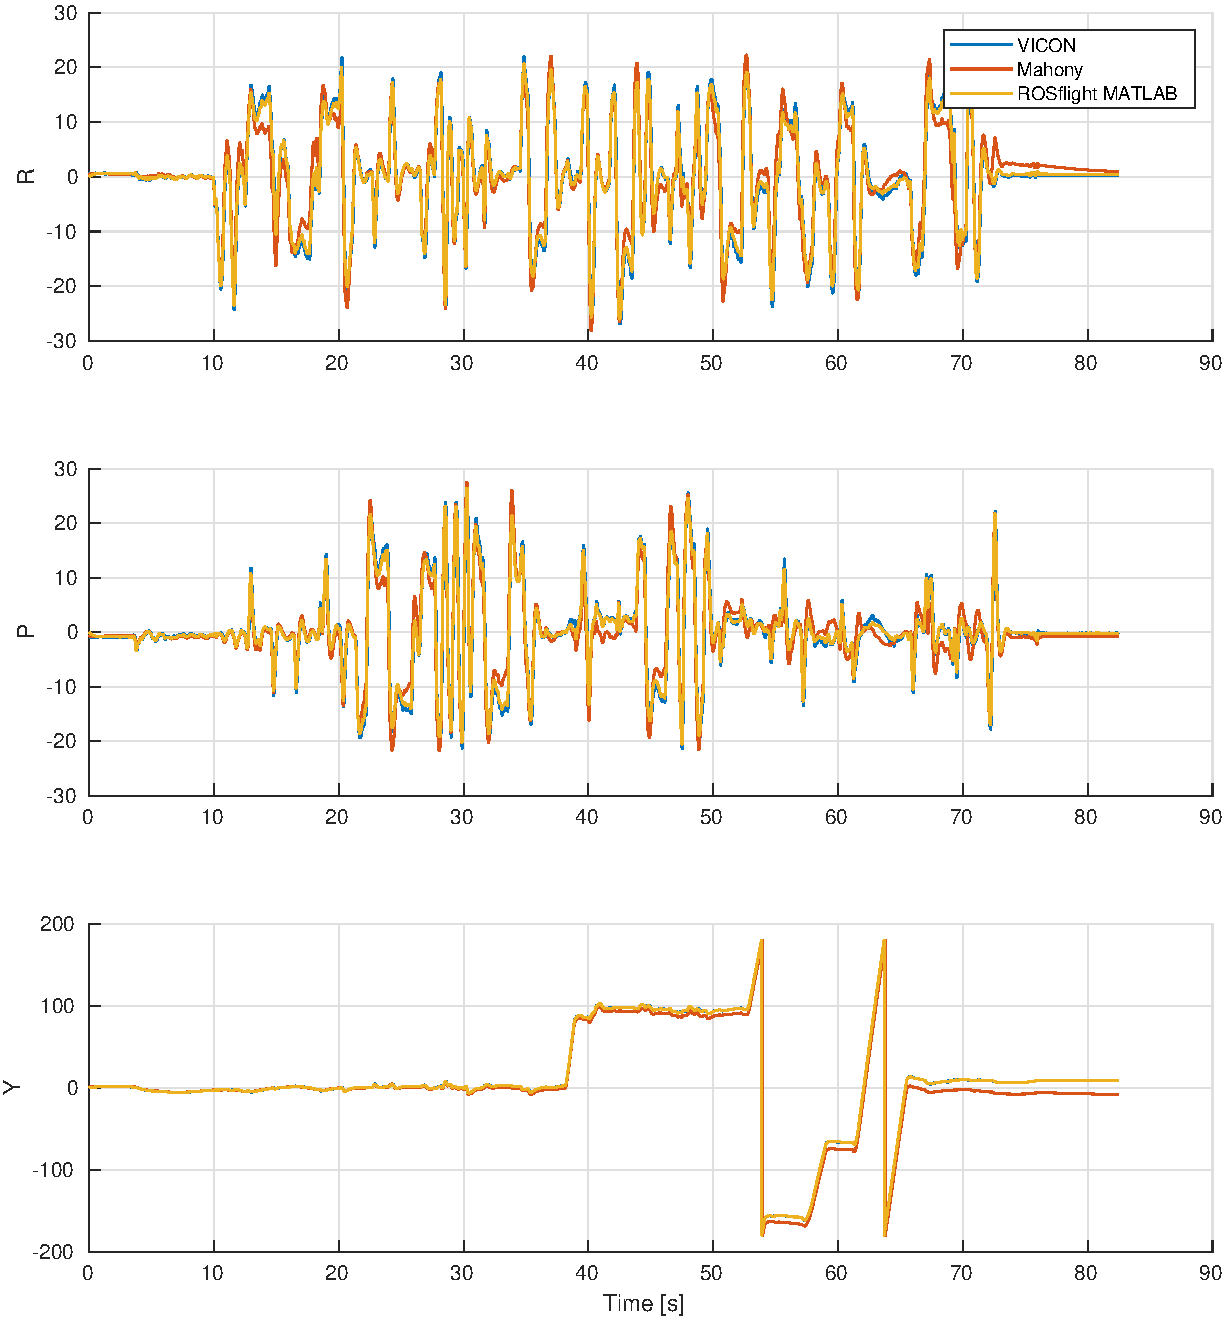
\includegraphics[width=\textwidth]{estrpy_accel_ext100.pdf}
    \caption{RPY estimates}
    \label{fig:scf_meas}
  \end{subfigure}\hfill
  \begin{subfigure}[t]{0.31\textwidth}
    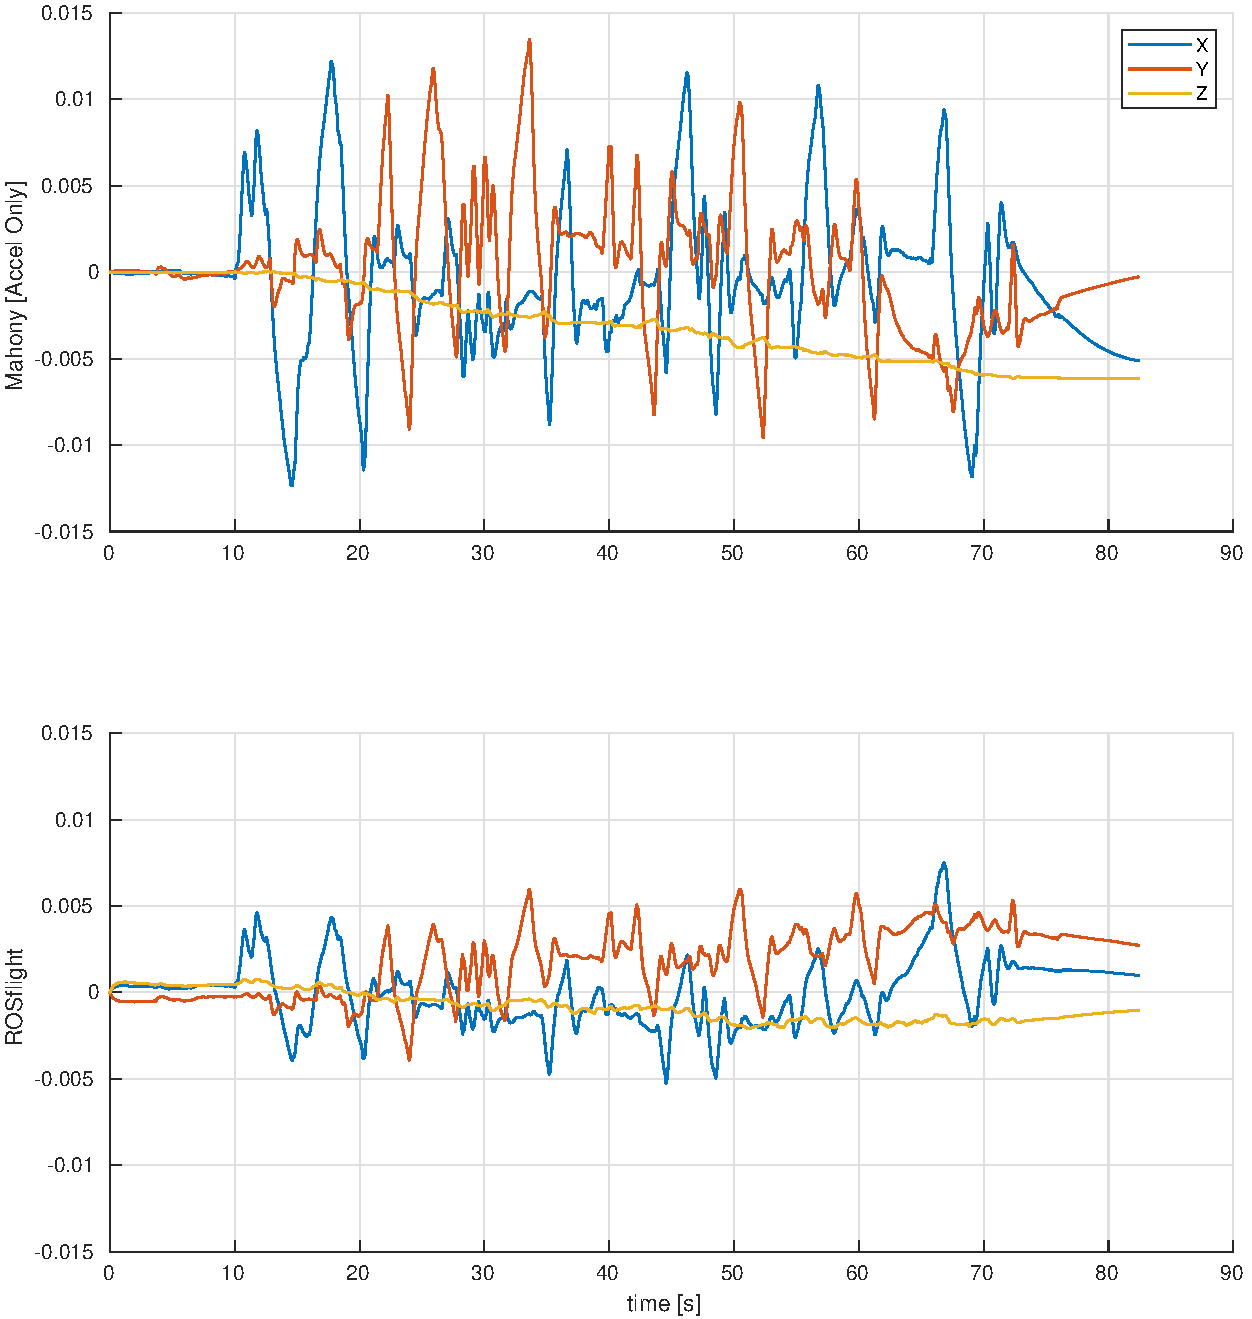
\includegraphics[width=\textwidth]{estbias_accel_ext100.pdf}
    \caption{Bias estimates}
    \label{fig:scf_est}
  \end{subfigure}\hfill
  \begin{subfigure}[t]{0.31\textwidth}
    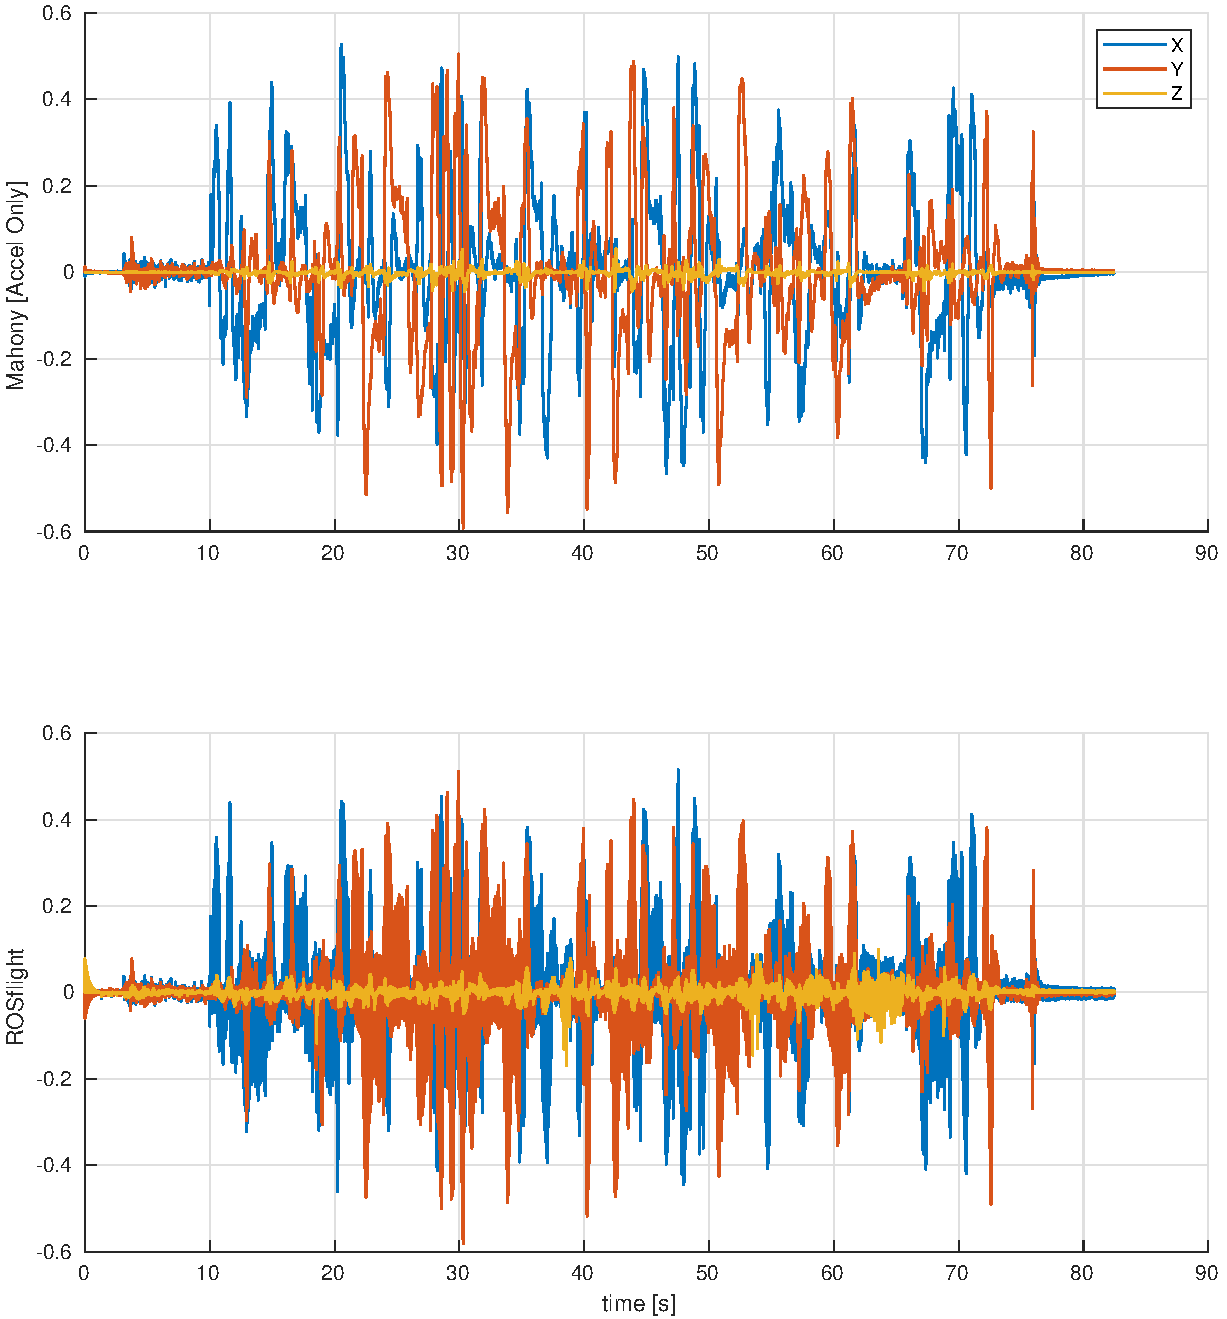
\includegraphics[width=\textwidth]{werr_accel_ext100.pdf}
    \caption{$\omega_\text{err}$}
    \label{fig:scf_bode}
  \end{subfigure}
  \caption{Results from Test 3.}
  \label{fig:scf}
\end{figure}

\subsubsection*{Test 4 - Gyro + External Attitude at 15 Hz}

\begin{figure}[H]
  \centering
  \begin{subfigure}[t]{0.31\textwidth}
    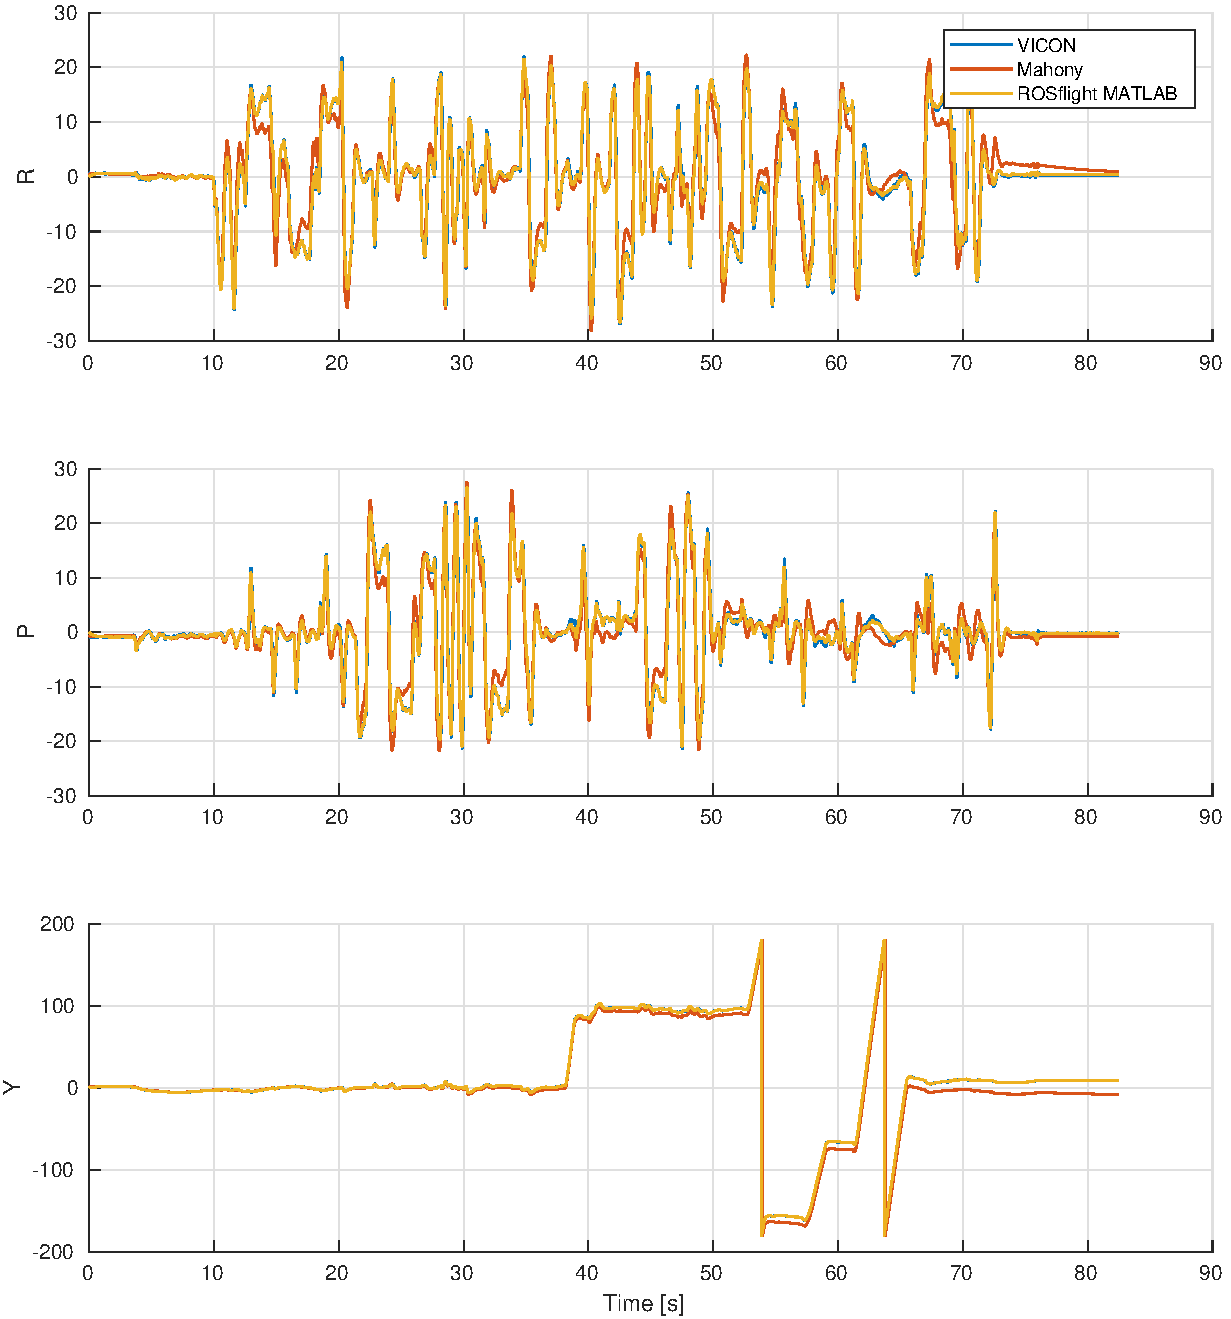
\includegraphics[width=\textwidth]{estrpy_ext15.pdf}
    \caption{RPY estimates}
    \label{fig:scf_meas}
  \end{subfigure}\hfill
  \begin{subfigure}[t]{0.31\textwidth}
    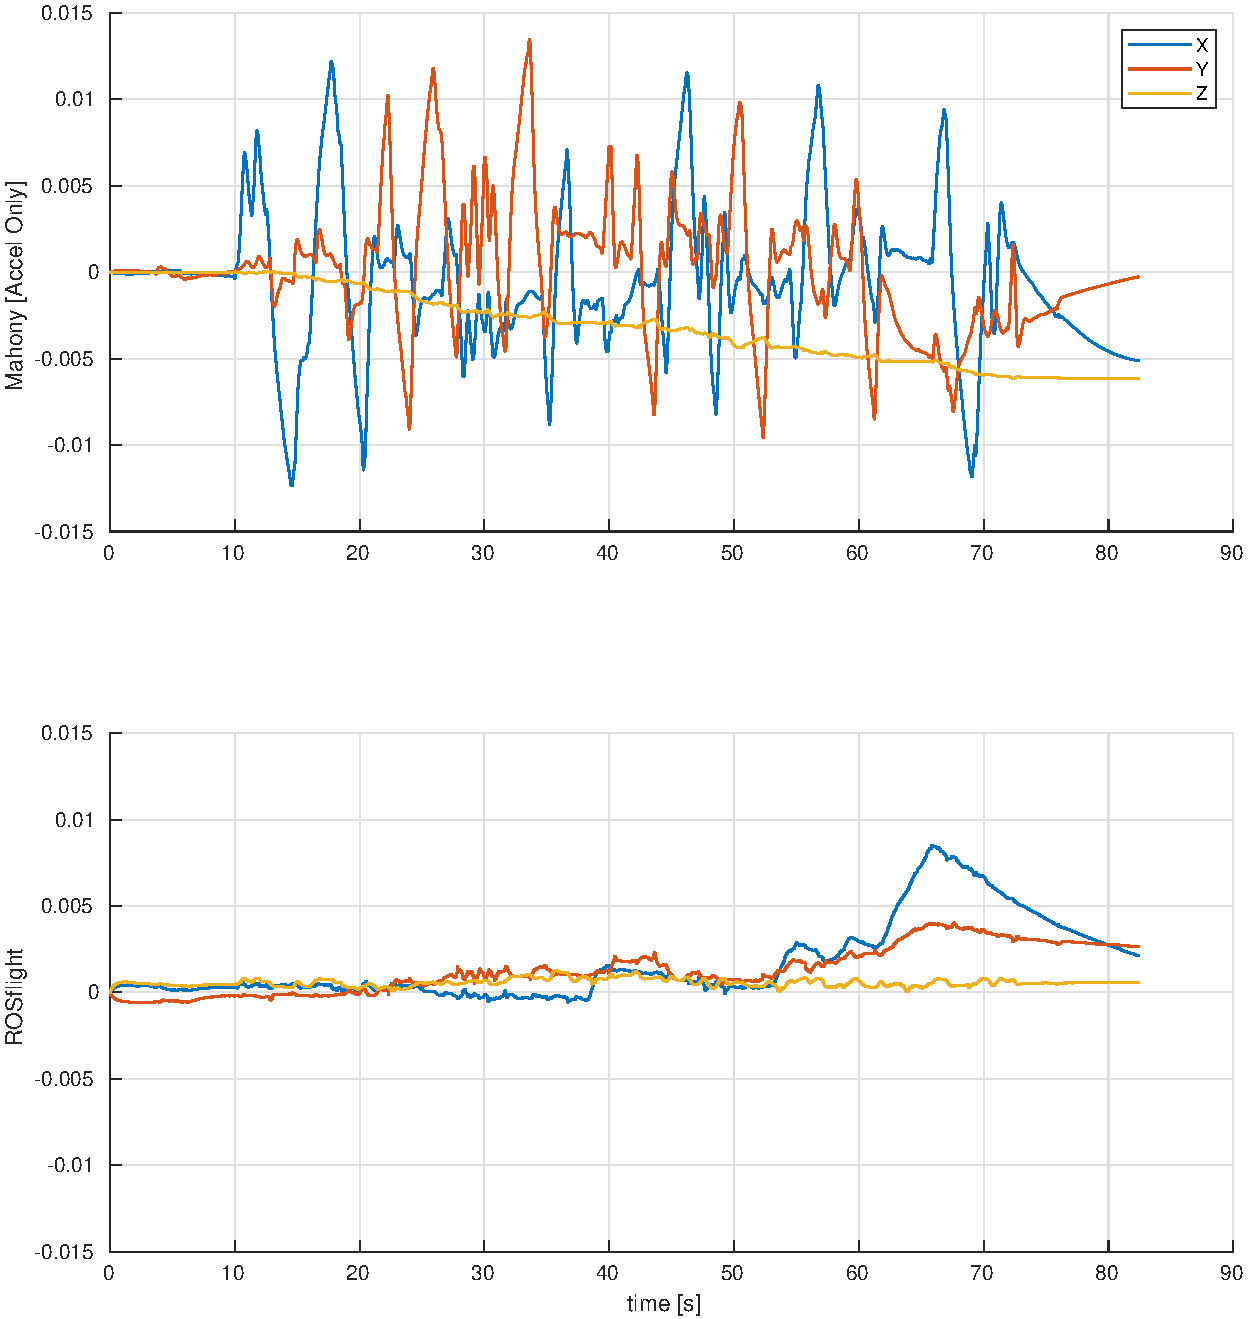
\includegraphics[width=\textwidth]{estbias_ext15.pdf}
    \caption{Bias estimates}
    \label{fig:scf_est}
  \end{subfigure}\hfill
  \begin{subfigure}[t]{0.31\textwidth}
    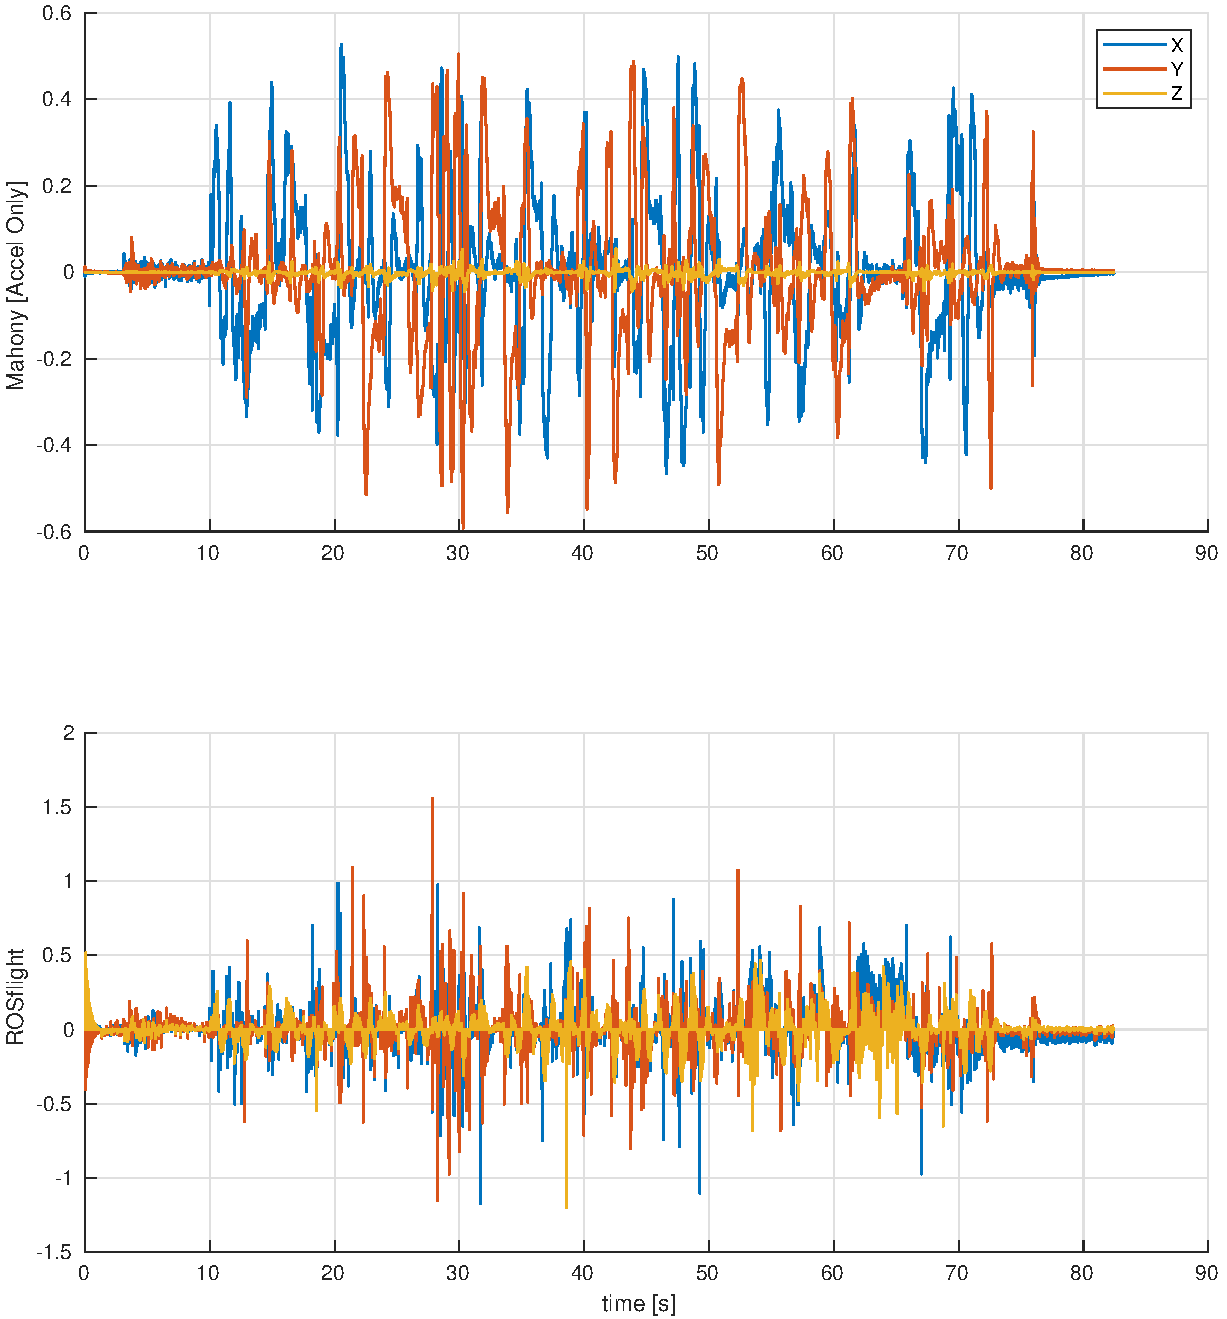
\includegraphics[width=\textwidth]{werr_ext15.pdf}
    \caption{$\omega_\text{err}$}
    \label{fig:scf_bode}
  \end{subfigure}
  \caption{Results from Test 4.}
  \label{fig:scf}
\end{figure}

\subsubsection*{Test 5 - Gyro + Accel + External Attitude at 15 Hz}

\begin{figure}[H]
  \centering
  \begin{subfigure}[t]{0.31\textwidth}
    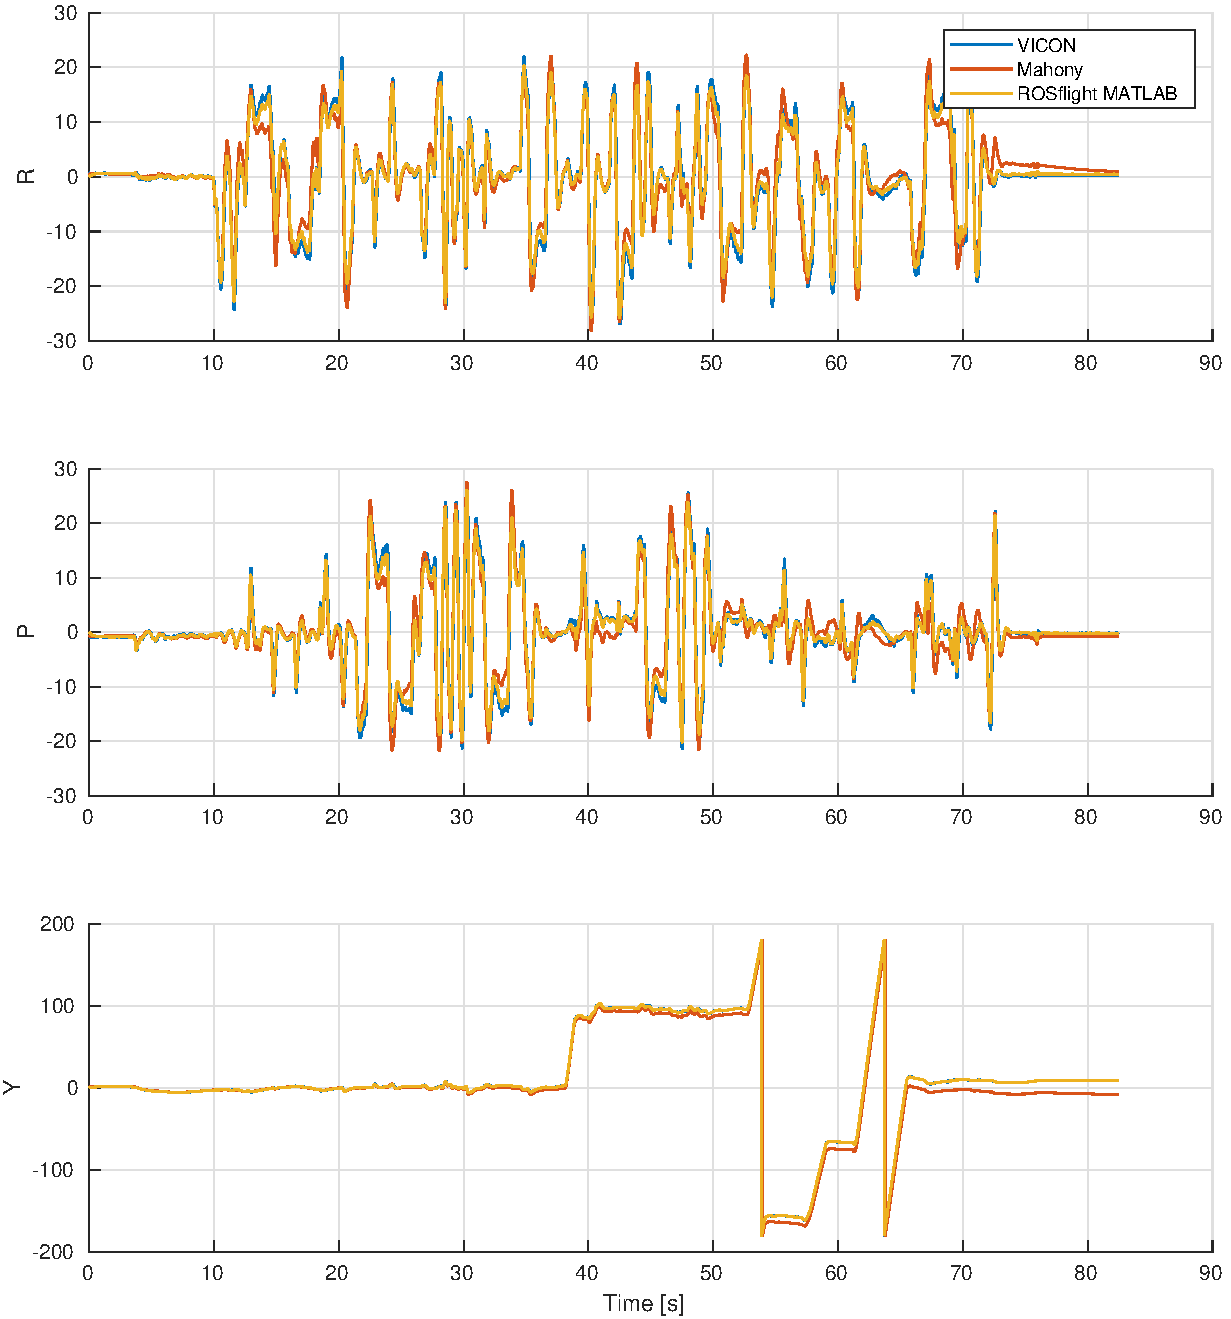
\includegraphics[width=\textwidth]{estrpy_accel_ext15.pdf}
    \caption{RPY estimates}
    \label{fig:scf_meas}
  \end{subfigure}\hfill
  \begin{subfigure}[t]{0.31\textwidth}
    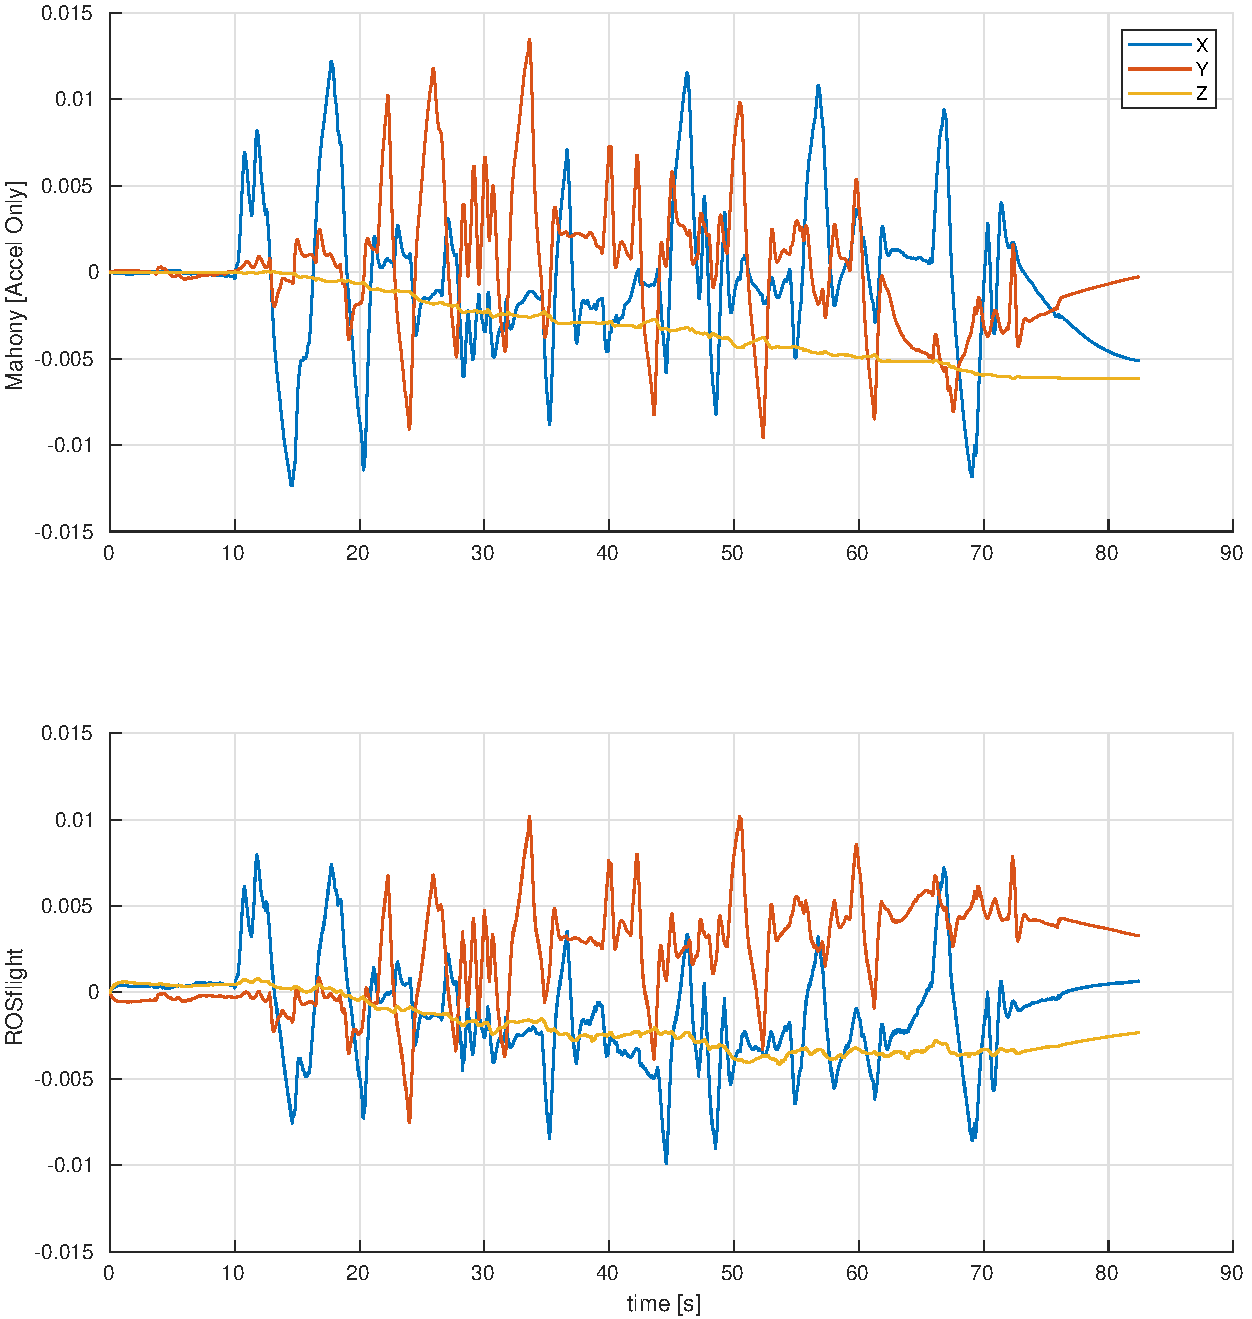
\includegraphics[width=\textwidth]{estbias_accel_ext15.pdf}
    \caption{Bias estimates}
    \label{fig:scf_est}
  \end{subfigure}\hfill
  \begin{subfigure}[t]{0.31\textwidth}
    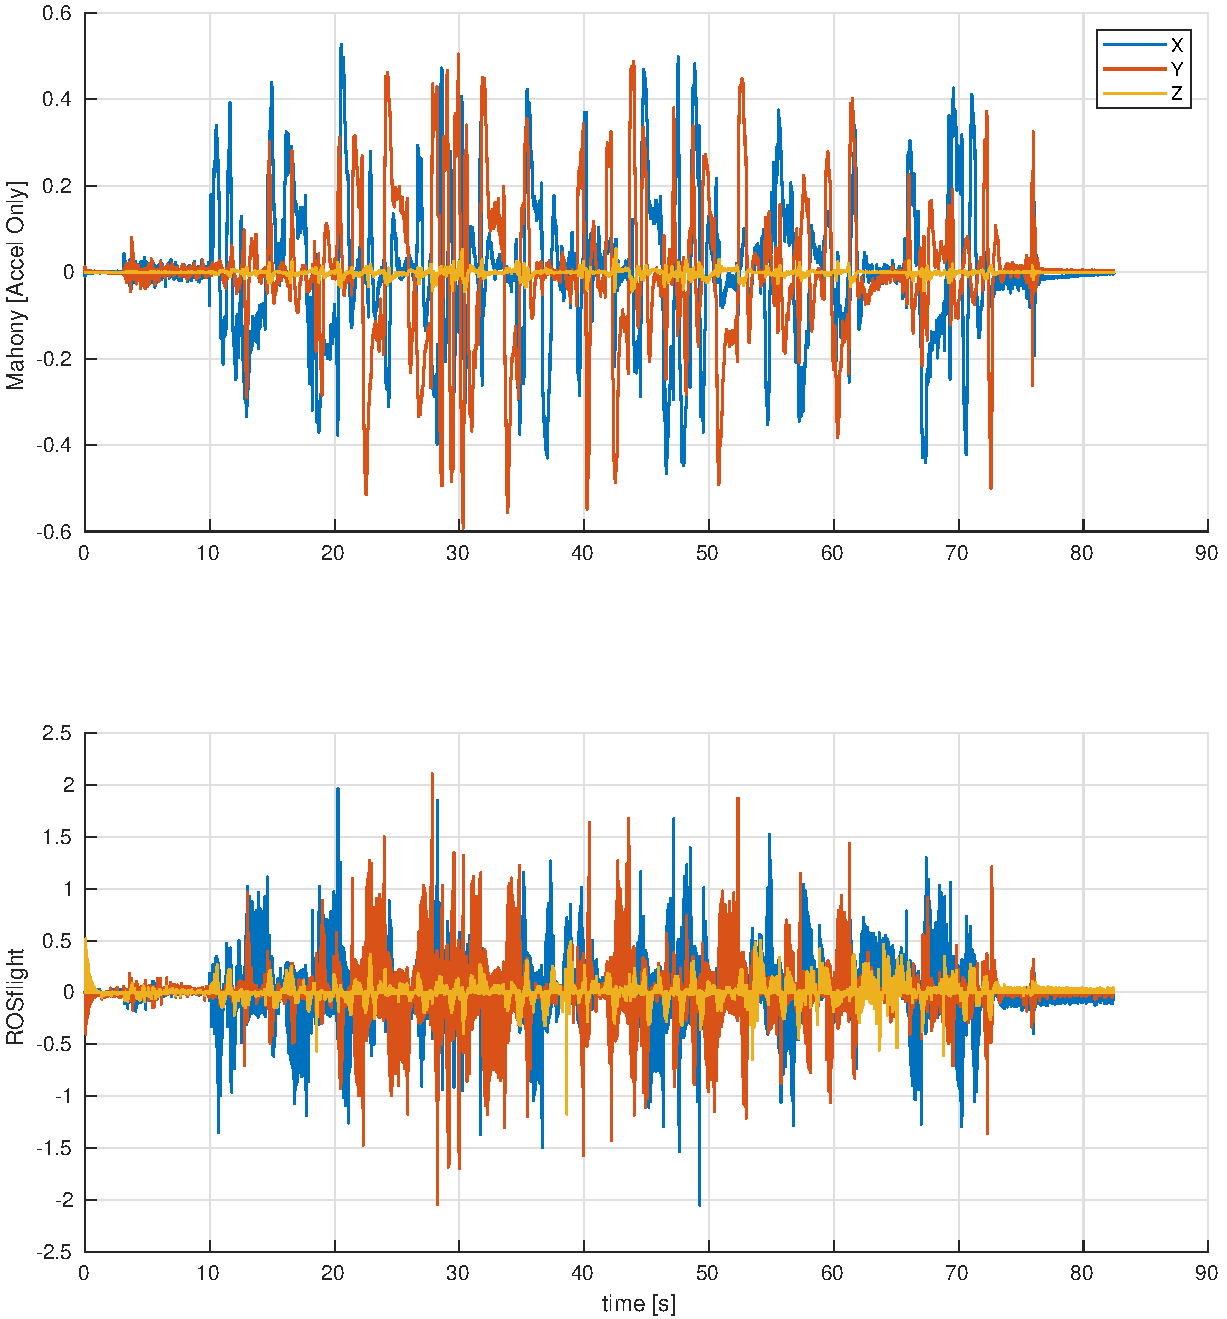
\includegraphics[width=\textwidth]{werr_accel_ext15.pdf}
    \caption{$\omega_\text{err}$}
    \label{fig:scf_bode}
  \end{subfigure}
  \caption{Results from Test 4.}
  \label{fig:scf}
\end{figure}

\section*{Things to Think About}
\begin{itemize}
  \item \href{https://arxiv.org/pdf/1602.07733.pdf}{Comparison of Attitude Estimation Techniques for Low-Cost UAVs}
  \item \href{https://en.wikipedia.org/wiki/Wahba%27s_problem}{Wahba's Problem}
  \item \href{https://www.analog.com/media/en/analog-dialogue/volume-46/number-3/articles/analyzing-frequency-response-of-inertial-mems.pdf}{Analyzing Frequency Response of Inertial MEMS}
  \item Keeping a Good Attitude: A Quaternion-Based Orientation Filter for IMUs and MARGs
  \item \href{https://ocw.mit.edu/courses/aeronautics-and-astronautics/16-333-aircraft-stability-and-control-fall-2004/lecture-notes/lecture_15.pdf}{16.333 Complementary Filters}
\end{itemize}

%%%%%%%%%%%%%%%%%%%%%%%%%%%%%%%%%%%%%%%%%%%%%%%%%%%%%%%%%%%%%%%%%%%%%%%%%%%%%%%
%%%%%%%%%%%%%%%%%%%%%%%%%%%%%%%%%%%%%%%%%%%%%%%%%%%%%%%%%%%%%%%%%%%%%%%%%%%%%%%
%%%%%%%%%%%%%%%%%%%%%%%%%%%%%%%%%%%%%%%%%%%%%%%%%%%%%%%%%%%%%%%%%%%%%%%%%%%%%%%
\bibliographystyle{IEEEtranN}
\bibliography{refs}

\end{document}
